\section{Introduction}

The objective of the mini-project is to go through the control design pipeline of a three-link 2D biped, in order to design and compare different controllers, both quantitatively (metrics of success) as well as qualitatively (gaits achieved).

\vspace{\baselineskip}

The control design pipeline consists of three steps.
The first is the modelling step, in which a model is chosen for the system of interest and implemented, along with means of visualizations.
In the case of this report, the model is the three-link 2D biped.
The second step is the control design step, which entails solving the equations of motion for the model as well as collision handling.
This is the simulation step.
Finally, the third step is the controller design step, in which gaits are achieved through controllers strategies.


\begin{center}
	\begin{tikzpicture}[auto]
		\node [block] (model) {Modelling};
		\node [block, below=of model] (control) {Control design};
		\node [block, below=of control] (simulation) {Simulation};

		\draw [->] (model) -- (control);
		\draw [->] (control) -- (simulation);
		\draw [->, rounded corners] (simulation) -- ++ (-2, 0) |- (control);
	\end{tikzpicture}
\end{center}

\vspace{\baselineskip}

The model for the theoretical legged robot studied in this robot is the three-link 2D biped, which can be represented as can be seen on Figure~\ref{fig::model} below :

\begin{figure}[H]
	\begin{center}
		\begin{tikzpicture}
			\begin{scope}[x={8cm},y={8cm}]
				% l = 0,447213
				% alpha = 8.999999999478607 deg
				% =0.5+sqrt(0.2^2+0.4^2)*sin(pi/20)
				% =0.4+sqrt(0.2^2+0.4^2)*cos(pi/20)
	
				\draw[-] (0,0)--(1,0);
	
				\draw[-,ultra thick] (0.3,0)--(0.5,0.4);
				\draw[-,ultra thick] (0.7,0)--(0.5,0.4);
				\draw[-,ultra thick] (0.5,0.4)--(0.5699596195707541,0.8417076540309386);
	
				\draw[dashed] (0.5,0.15)--(0.5,0.8);
				\draw[dashed] (0.7,0)--(0.7,0.25);
	
				\draw[->,ultra thick, red] (0.7,0)--(0.8,0) node[above]{$x$};
				\draw[->,ultra thick, red] (0.7,0)--(0.7,0.1) node[right]{$y$};
	
				\draw [->,thick,domain=-90:-116.5650512] plot ({0.5+0.15*cos(\x)}, {0.4+0.15*sin(\x)});
				\draw [->,thick,domain=90:116.5650512] plot ({0.7+0.15*cos(\x)}, {0.15*sin(\x)});
				\draw [->,thick,domain=90:81.00000000052139] plot ({0.5+0.3*cos(\x)}, {0.4+0.3*sin(\x)});
	
				\node at (0.4,0.2) [circle,fill,inner sep=1]{.};
				\node at (0.6,0.2) [circle,fill,inner sep=1]{.};
				\node at (0.5349798097853771,0.6208538270154693) [circle,fill,inner sep=1]{.};
	
				\node[text width=0mm] at (0.63,0.2) {$q_1$};
				\node[text width=0mm] at (0.43,0.2) {$q_2$};
				\node[text width=0mm] at (0.51,0.76) {$q_3$};
	
				\node[text width=0mm] at (0.55,0.16) {$m_1$};
				\node[text width=0mm] at (0.32,0.2) {$m_2$};
				\node[text width=0mm] at (0.56,0.62) {$m_3$};
	
				\node[text width=0mm] at (0.58,0.33) {$\dfrac{l_1}{2}$};
				\node[text width=0mm] at (0.38,0.33) {$\dfrac{l_2}{2}$};
				\node[text width=0mm] at (0.55,0.5) {$\dfrac{l_3}{2}$};
			\end{scope}
		\end{tikzpicture}
	\end{center}
	\caption{Representation of the three-link 2D biped model.}
	\label{fig::model}
\end{figure}

\newpage
